\documentclass[tikz,crop]{standalone}

\usepackage{xcolor}
\definecolor{cps}{RGB}{165,0,38}
\definecolor{feed}{RGB}{215,48,39}
\definecolor{wireless}{RGB}{244,109,67}
\definecolor{safety}{RGB}{253,174,97}
\definecolor{sec}{RGB}{254,224,144}
\definecolor{method}{RGB}{224,243,248}
\definecolor{spec}{RGB}{171,217,233}
\definecolor{app}{RGB}{116,173,209}
\definecolor{vv}{RGB}{69,117,180}

\usepackage{tikz}
\usetikzlibrary{shapes, shapes.geometric,arrows, backgrounds, calc, hobby, positioning}

\tikzset{vertex style/.style={
    % draw=#1,
    % thick,
    fill=#1!70,
    text=black,
    rounded rectangle,
    minimum width=2cm,
    minimum height=0.75cm,
    font=\normalsize,
    outer sep=3pt, % the usage of this option will be clear later on
  },
}

\tikzset{
  text style/.style={
    sloped, % the text will be parallel to the connection 
    text=black,
    font=\footnotesize,
    above
  }
}

\begin{document}

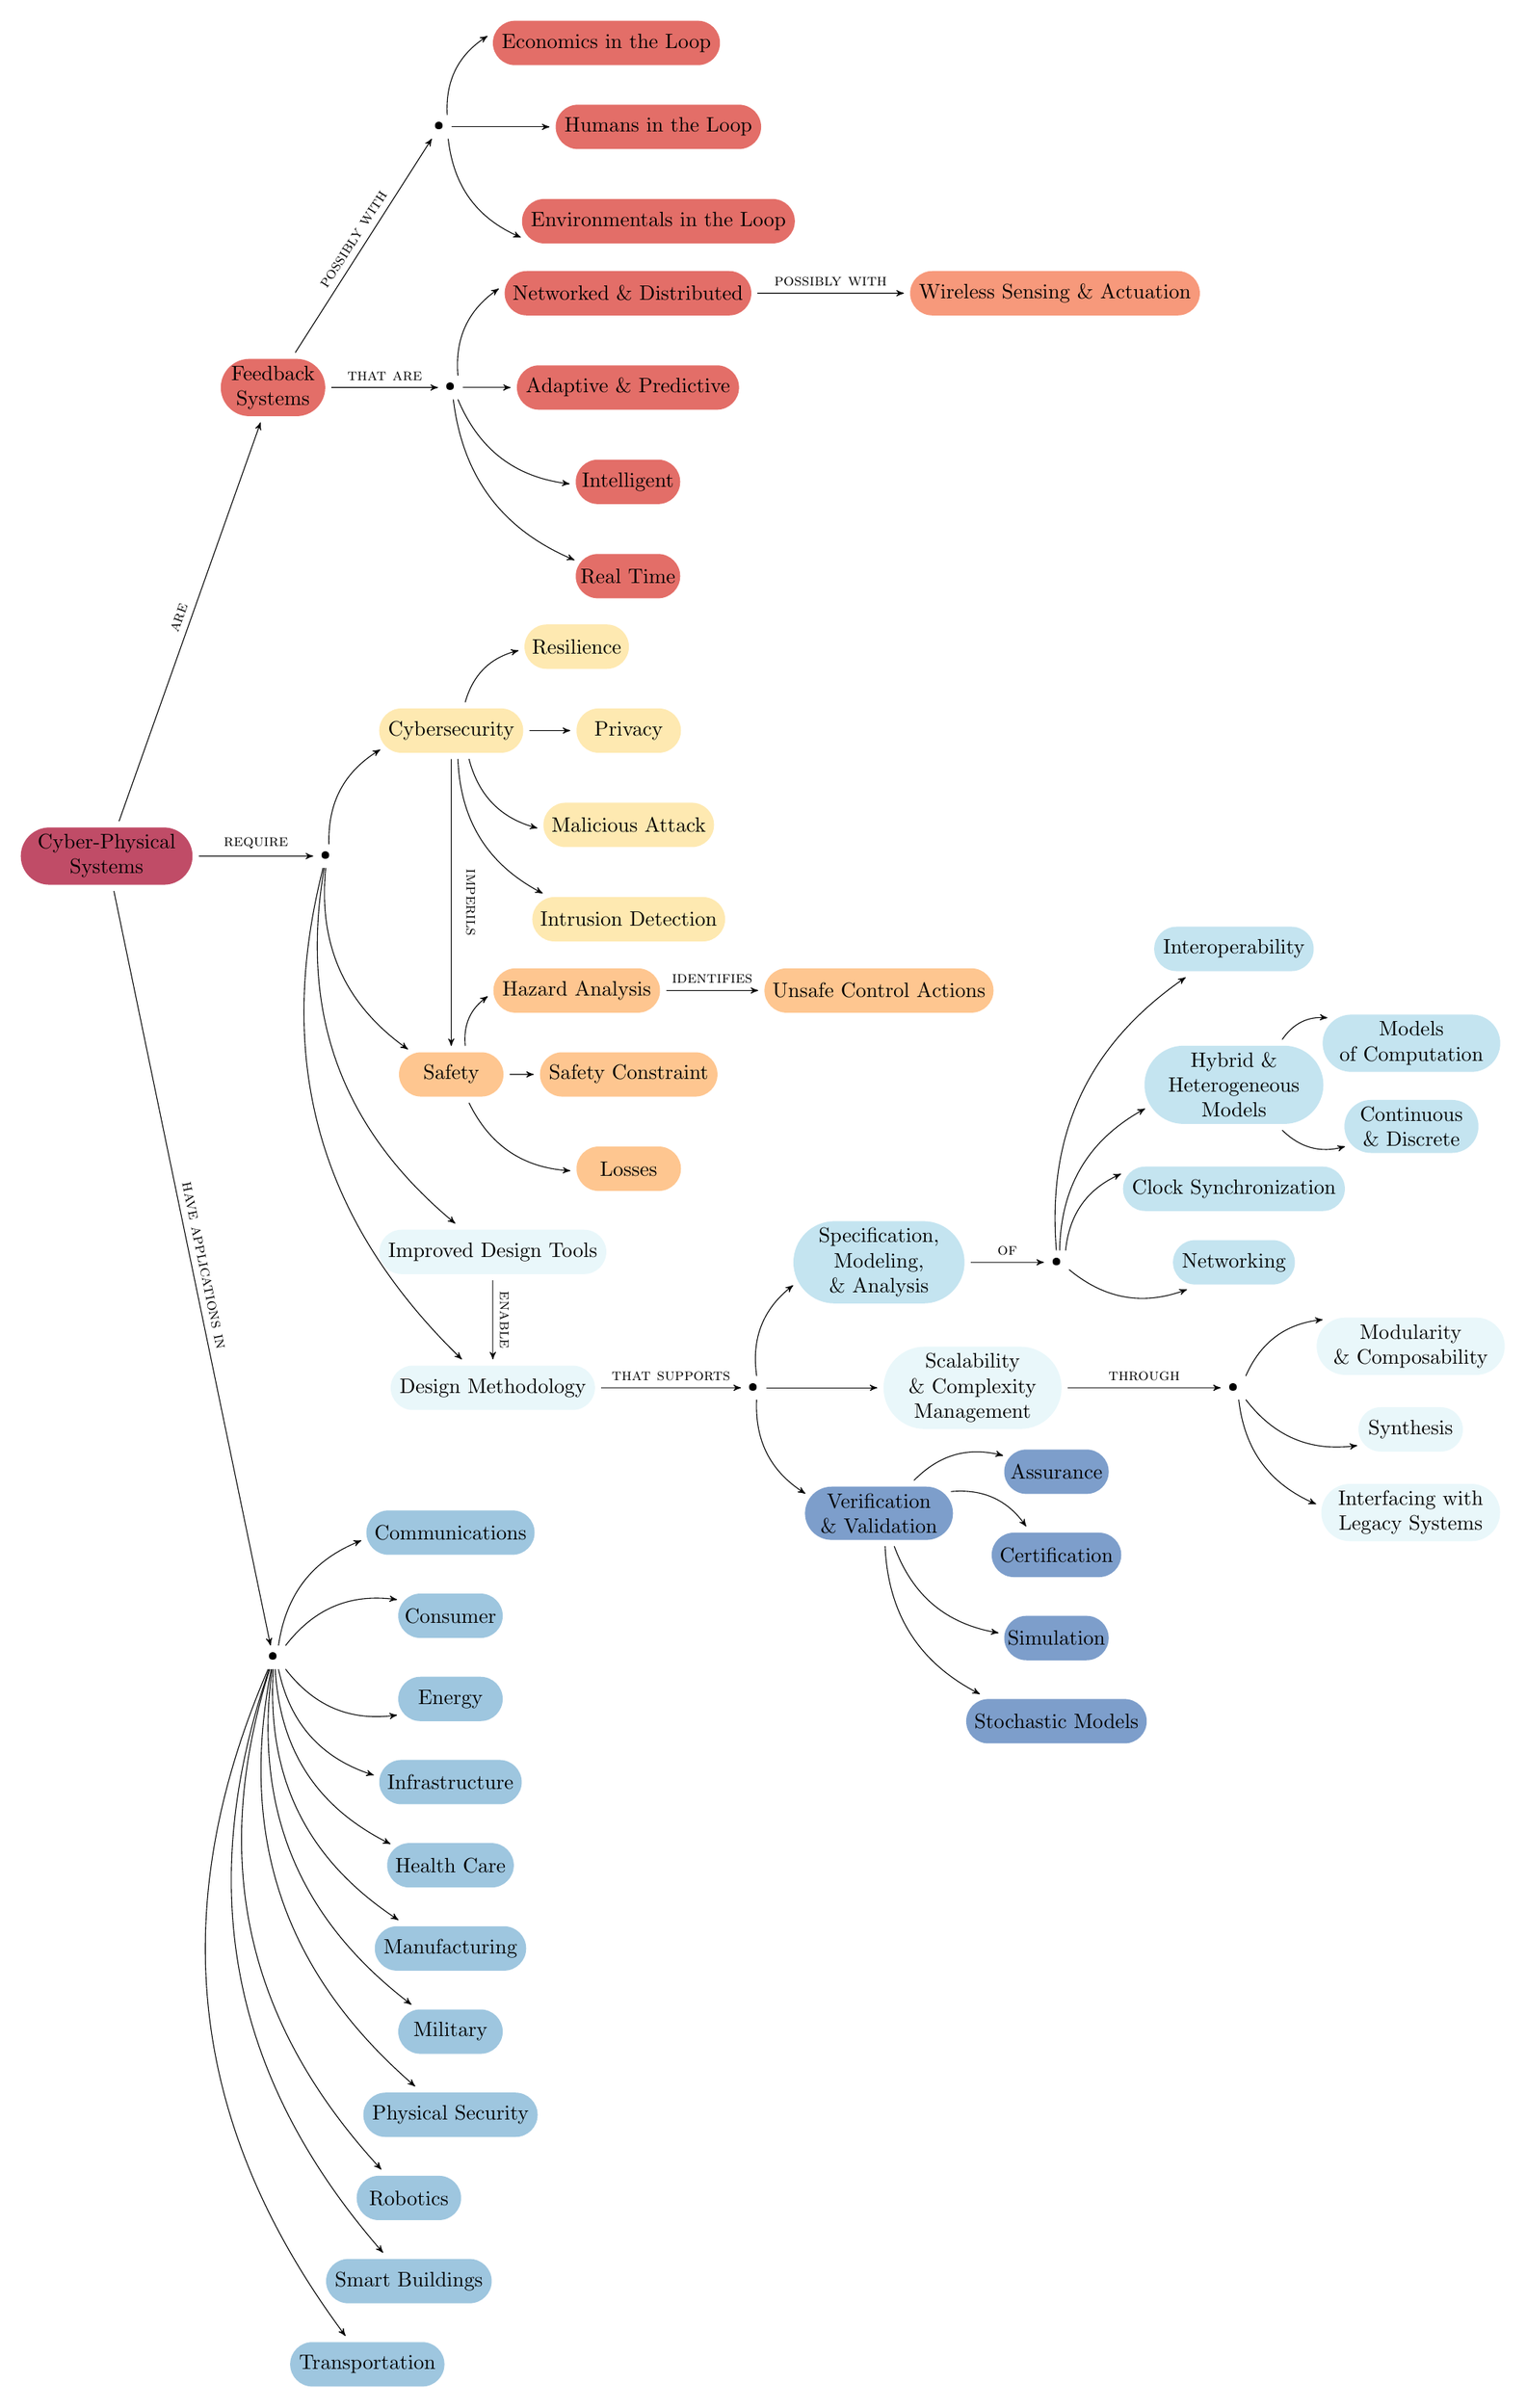
\begin{tikzpicture}[node distance=3cm and 6cm,>=stealth']
% main node
 \node[vertex style=cps, align=center] (cps) {Cyber-Physical\\ Systems};

% are
 \node[vertex style=feed, above of=cps,xshift=8em, yshift=14em, align = center] (fb) {Feedback\\ Systems}
 edge [<-] node[text style,above]{\textsc{are}} (cps);
 
 \node[above of=fb, xshift=8em, yshift=4em] (fb-bullet) {•}
 edge [<-] node[text style, above]{\textsc{possibly with}} (fb);
 \node[vertex style=feed,above right of=fb-bullet, yshift=-2em, xshift=2em] (econ) {Economics in the Loop}
 edge [<-, bend right] (fb-bullet);
 \node[vertex style=feed, right of=fb-bullet, xshift=2em] (human) {Humans in the Loop}
 edge [<-] (fb-bullet);
 \node[vertex style=feed, below of=human, yshift=4em] (env) {Environmentals in the Loop}
 edge [<-, bend left] (fb-bullet);
 
  \node[right of=fb] (fb-bullet2) {•}
  edge [<-] node[text style, above]{\textsc{that are}} (fb);
  \node[vertex style = feed, right of=fb-bullet2] (ad) {Adaptive \& Predictive}
  edge [<-] (fb-bullet2);
  \node[vertex style = feed, above of = ad, yshift=-4em] (network) {Networked \& Distributed}
  edge [<-, bend right] (fb-bullet2);
  \node[vertex style = wireless, right of = network, xshift=12em] {Wireless Sensing \& Actuation}
    edge [<-] node[text style, above]{\textsc{possibly with}} (network);
  \node[vertex style = feed, below of = ad, yshift = 4em] (intel) {Intelligent}
  edge[<-, bend left] (fb-bullet2);
    \node[vertex style = feed, below of = intel, yshift = 4em] {Real Time}
  edge[<-, bend left] (fb-bullet2);
  
 % require
\node[right of = cps, xshift=2em] (req-bullet) {•}
 edge [<-] node[text style, above]{\textsc{require}} (cps);
 \node[vertex style=sec, above right of = req-bullet] (sec) {Cybersecurity}
 edge [<-, bend right] (req-bullet);
    \node[vertex style=sec, above right of = sec, yshift=-2em] {Resilience}
     edge [<-, bend right] (sec);
    \node[vertex style=sec, right of = sec]  (priv) {Privacy}
     edge [<-] (sec);
    \node[vertex style=sec, below of = priv, yshift=4em]  (ma) {Malicious Attack}
     edge [<-, bend left] (sec);
    \node[vertex style=sec, below of = ma, yshift=4em]  {Intrusion Detection}
     edge [<-, bend left] (sec);
 \node[vertex style=safety, below of = sec, yshift=-8em] (safety) {Safety}
 edge [<-, bend left] (req-bullet)
 edge [<-] node[text style, below, rotate=180, yshift=1.5em]{\textsc{imperils}} (sec);
    \node[vertex style=safety, above right of = safety, yshift=-2em] (hazop) {Hazard Analysis}
     edge [<-, bend right] (safety);
        \node[vertex style=safety, right of = hazop, xshift=6em] {Unsafe Control Actions}
        edge [<-] node[text style, above]{\textsc{identifies}} (hazop);
    \node[vertex style=safety, right of = safety] (sc) {Safety Constraint}
     edge [<-] (safety);
    \node[vertex style=safety, below of = sc, yshift=4em] {Losses}
     edge [<-, bend left] (safety);
 
  \node[vertex style=method, below of = safety, xshift=2em] (tools) {Improved Design Tools}
 edge [<-, bend left] (req-bullet);
 
 \node[vertex style=method, below of = tools, yshift=2em] (method) {Design Methodology}
 edge [<-, bend left] (req-bullet)
 
 edge [<-] node[text style, above] {\textsc{enable}} (tools);

\node[right of = method, xshift=4em] (method-bullet) {•}
 edge [<-] node[text style, above] {\textsc{that supports}} (method);
 \node[vertex style=spec, above right of = method-bullet, align=center] (spec) {Specification,\\
 Modeling,\\
 \& Analysis}
 edge [<-, bend right] (method-bullet);
    \node[right of = spec] (spec-bullet) {•}
    edge [<-] node[text style, above] {\textsc{of}} (spec);
        \node[vertex style = spec, right of = spec-bullet] (networking) {Networking}
        edge [<-, bend left] (spec-bullet);
        \node[vertex style = spec, above of = networking, align=center] (hybrid) {Hybrid \&\\ Heterogeneous\\ Models}
        edge [<-, bend right] (spec-bullet);
            \node[vertex style = spec, right of = hybrid, align=center, yshift=-2em] {Continuous\\ \& Discrete}
            edge [<-, bend left] (hybrid);
            \node[vertex style = spec, right of = hybrid, align=center, yshift=2em] {Models\\ of Computation}
            edge [<-, bend right] (hybrid);
        \node[vertex style = spec, above of = hybrid, align=center, yshift=-2em] (inter) {Interoperability}
        edge [<-, bend right] (spec-bullet);
        \node[vertex style = spec, above of = networking, align=center, yshift=-5em]  {Clock Synchronization}
        edge [<-, bend right] (spec-bullet);     
 \node[vertex style=method, right of = method-bullet, align=center, xshift=2em] (comp) {Scalability\\ \& Complexity\\ Management}
 edge [<-] (method-bullet);
     \node[right of = comp, xshift=4em] (comp-bullet) {•}
     edge [<-] node[text style, above] {\textsc{through}} (comp);
        \node[vertex style = method, right of = comp-bullet, align=center, yshift=2em] {Modularity\\ \& Composability}
        edge [<-, bend right] (comp-bullet);
        \node[vertex style = method, right of = comp-bullet, align=center, yshift=-2em] {Synthesis}
        edge [<-, bend left] (comp-bullet);
         \node[vertex style = method, right of = comp-bullet, align=center, yshift=-6em] {Interfacing with\\ Legacy Systems}
        edge [<-, bend left] (comp-bullet);
 \node[vertex style=vv, below right of = method-bullet, align=center] (vv) {Verification\\ \& Validation}
 edge [<-, bend left] (method-bullet);
        \node[vertex style = vv, right of = vv, align=center, yshift=2em] {Assurance}
        edge [<-, bend right] (vv);
        \node[vertex style = vv, right of = vv, align=center, yshift=-2em] {Certification}
        edge [<-, bend right] (vv);
        \node[vertex style = vv, right of = vv, align=center, yshift=-6em] {Simulation}
        edge [<-, bend left] (vv);
        \node[vertex style = vv, right of = vv, align=center, yshift=-10em] {Stochastic Models}
        edge [<-, bend left] (vv);

 % applications
 \node[below of = cps, xshift=8em, yshift=-30em] (app-bullet) {•}
 edge [<-] node[text style, above]{\textsc{have applications in}} (cps);
        \node[vertex style = app, right of = app-bullet, align=center, yshift=6em] {Communications}
        edge [<-, bend right] (app-bullet);
        \node[vertex style = app, right of = app-bullet, align=center, yshift=2em] {Consumer}
        edge [<-, bend right] (app-bullet);
        \node[vertex style = app, right of = app-bullet, align=center, yshift=-2em] {Energy}
        edge [<-, bend left] (app-bullet);
        \node[vertex style = app, right of = app-bullet, align=center, yshift=-6em] {Infrastructure}
        edge [<-, bend left] (app-bullet);
        \node[vertex style = app, right of = app-bullet, align=center, yshift=-10em] {Health Care}
        edge [<-, bend left] (app-bullet);
        \node[vertex style = app, right of = app-bullet, align=center, yshift=-14em] {Manufacturing}
        edge [<-, bend left] (app-bullet);
        \node[vertex style = app, right of = app-bullet, align=center, yshift=-18em] {Military}
        edge [<-, bend left] (app-bullet);
        \node[vertex style = app, right of = app-bullet, align=center, yshift=-22em] {Physical Security}
        edge [<-, bend left] (app-bullet);
        \node[vertex style = app, right of = app-bullet, align=center, yshift=-26em, xshift=-2em] {Robotics}
        edge [<-, bend left] (app-bullet);
        \node[vertex style = app, right of = app-bullet, align=center, yshift=-30em, xshift=-2em] {Smart Buildings}
        edge [<-, bend left] (app-bullet);
        \node[vertex style = app, right of = app-bullet, align=center, yshift=-34em, xshift=-4em] {Transportation}
        edge [<-, bend left] (app-bullet);
\end{tikzpicture}
\end{document}